%%%%%%%%%%%%%%%%%%%%%%%%%%%%%%%%%%%%%%%%%%%%%%%%%%%%%%%%%%%%%%%%%%%%%%%%%%%%%
%%%
%%% File: utthesis2.doc, version 2.0jab, February 2002
%%%
%%% Based on: utthesis.doc, version 2.0, January 1995
%%% =============================================
%%% Copyright (c) 1995 by Dinesh Das.  All rights reserved.
%%% This file is free and can be modified or distributed as long as
%%% you meet the following conditions:
%%%
%%% (1) This copyright notice is kept intact on all modified copies.
%%% (2) If you modify this file, you MUST NOT use the original file name.
%%%
%%% This file contains a template that can be used with the package
%%% utthesis.sty and LaTeX2e to produce a thesis that meets the requirements
%%% of the Graduate School of The University of Texas at Austin.
%%%
%%% All of the commands defined by utthesis.sty have default values (see
%%% the file utthesis.sty for these values).  Thus, theoretically, you
%%% don't need to define values for any of them; you can run this file
%%% through LaTeX2e and produce an acceptable thesis, without any text.
%%% However, you probably want to set at least some of the macros (like
%%% \thesisauthor).  In that case, replace "..." with appropriate values,
%%% and uncomment the line (by removing the leading %'s).
%%%
%%%%%%%%%%%%%%%%%%%%%%%%%%%%%%%%%%%%%%%%%%%%%%%%%%%%%%%%%%%%%%%%%%%%%%%%%%%%%

\documentclass[a4paper, 12pt, oneside]{report}         %% LaTeX2e document.
\usepackage {tcdthesis}              %% Preamble.
\usepackage{graphicx,color}
\usepackage{anysize}
\usepackage{amsmath}
\usepackage[bibstyle= nature, citestyle=numeric-comp, sorting=none]{biblatex}

\bibliography{collection}
\mastersthesis                     %% Uncomment one of these; if you don't
%\phdthesis                         %% use either, the default is \phdthesis.

\thesisdraft                       %% Uncomment this if you want a draft
                                     %% version; this will print a timestamp
                                     %% on each page of your thesis.

\leftchapter                       %% Uncomment one of these if you want
%\centerchapter                      %% left-justified, centered or
% \rightchapter                      %% right-justified chapter headings.
                                     %% Chapter headings includes the
                                     %% Contents, Acknowledgments, Lists
                                     %% of Tables and Figures and the Vita.
                                     %% The default is \centerchapter.

% \singlespace                       %% Uncomment one of these if you want
% \oneandhalfspace                   %% single-spacing, space-and-a-half
 \doublespace                       %% or double-spacing; the default is
                                     %% \oneandhalfspace, which is the
                                     %% minimum spacing accepted by the
                                     %% Graduate School.

\renewcommand{\thesisauthor}{Gu Juntao}            %% Your official UT name.
\renewcommand{\thesismonth}{September}                  %% Your month of graduation.
\renewcommand{\thesisyear}{2013}                      %% Your year of graduation.
\renewcommand{\thesistitle}{\large{} \\ \LARGE{Secure Dropbox}}            %% The title of your thesis; use mixed-case.
\renewcommand{\thesisauthorpreviousdegrees}{B.Sc.}  %% Your previous degrees, abbreviated; separate multiple degrees by commas.
\renewcommand{\thesissupervisor}{Tewari Hitesh}      %% Your thesis supervisor; use mixed-case and don't use any titles or degrees.
% \renewcommand{\thesiscosupervisor}{}                %% Your PhD. thesis co-supervisor; if any.

% \renewcommand{\thesiscommitteemembera}{}
% \renewcommand{\thesiscommitteememberb}{}
% \renewcommand{\thesiscommitteememberc}{}
% \renewcommand{\thesiscommitteememberd}{}
% \renewcommand{\thesiscommitteemembere}{}
% \renewcommand{\thesiscommitteememberf}{}
% \renewcommand{\thesiscommitteememberg}{}
% \renewcommand{\thesiscommitteememberh}{}
% \renewcommand{\thesiscommitteememberi}{}

\renewcommand{\thesisauthoraddress}{Dublin, Ireland}

%\renewcommand{\thesisdedication}{...}     %% Your dedication, if you have one; use "\\" for linebreaks.


%%%%%%%%%%%%%%%%%%%%%%%%%%%%%%%%%%%%%%%%%%%%%%%%%%%%%%%%%%%%%%%%%%%%%%%%%%%%%
%%%
%%% The following commands are all optional, but useful if your requirements
%%% are different from the default values in utthesis.sty.  To use them,
%%% simply uncomment (remove the leading %) the line(s).

% \renewcommand{\thesiscommitteesize}{...}
                                     %% Uncomment this only if your thesis
                                     %% committee does NOT have 5 members
                                     %% for \phdthesis or 2 for \mastersthesis.
                                     %% Replace the "..." with the correct
                                     %% number of members.

\renewcommand{\thesisdegree}{Master of Science in Computer Science}  %% Uncomment this only if your thesis
                                     %% degree is NOT "DOCTOR OF PHILOSOPHY"
                                     %% for \phdthesis or "MASTER OF ARTS"
                                     %% for \mastersthesis.  Provide the
                                     %% correct FULL OFFICIAL name of
                                     %% the degree.

\renewcommand{\thesisdegreeabbreviation}{M.Sc.}
                                     %% Use this if you also use the above
                                     %% command; provide the OFFICIAL
                                     %% abbreviation of your thesis degree.

\renewcommand{\thesistype}{Dissertation}    %% Use this ONLY if your thesis type
                                     %% is NOT "Dissertation" for \phdthesis
                                     %% or "Thesis" for \mastersthesis.
                                     %% Provide the OFFICIAL type of the
                                     %% thesis; use mixed-case.

% \renewcommand{\thesistypist}{...}  %% Use this to specify the name of
                                     %% the thesis typist if it is anything
                                     %% other than "the author".

%%%
%%%%%%%%%%%%%%%%%%%%%%%%%%%%%%%%%%%%%%%%%%%%%%%%%%%%%%%%%%%%%%%%%%%%%%%%%%%%%

\begin{document}                                  %% BEGIN THE DOCUMENT

\thesistitlepage                                  %% Generate the title page.

\thesisdeclarationpage    			  %% Generate the declaration page.

\thesispermissionpage				  %% Generate the copyright permission page

%\thesisdedicationpage                             %% Generate the dedication page.

\begin{thesisacknowledgments}                     %% Use this to write your
			                          %% acknowledgments; it can be anything
Give many thanks and stuff...

\end{thesisacknowledgments}                       %% allowed in LaTeX2e par-mode.

\begin{thesisabstract}

Recently there have been increasing requirements about utilizing cloud technology for data maintaining and management especially when reliable, stable data storage and remote data access required. Since the cloud storage service is usually designed to be available to users over the Internet, it essentially facilitates the data sharing as well. However, security concerns are growing as the most commonly cited reason why users, particularly those enterprise users who are information confidentiality critical, are not interested in SaaS \cite{kamara2010cryptographic}, of which cloud storage services like Dropbox or Google Drive are typical instances. The use of those cloud storage service is actually exposing the sensitive data to the service vendors.
This research project aims to investigate the feasibility of solving the data exposing issue and achieving the goal of secure data sharing via encryption approaches. It was decided to develop an application to explore this topic. A client end encryption tool would be implemented based on Python and Python accredited cryptography related modules. What is more, a key management system (KMS) with features of file encryption management, user profile management and sharing information management would be deployed to realize the function of everywhere use and secure data sharing. Dropbox would be selected as the instance of SaaS cloud storage service for demonstration purpose so that Dropbox core API would be used.
The result of the project indicated the idea of the hybrid application of symmetric and asymmetric cryptography algorithm could effectively protect the data stored on Dropbox and potentially could be implemented. The user testing session in the end of the project also strongly indicated that the encryption tool Secure Dropbox could tremendously gain users’ confidence in terms of storing their confidential data on cloud storage service like Dropbox.

\end{thesisabstract}

\tableofcontents                                  %% Generate table of contents.
\listoftables                                     %% Uncomment this to generate list of tables.
\listoffigures                                    %% Uncomment this to generate list of figures.

%%
%% Include thesis chapters here...
%%
  \chapter{Introduction}
Cloud computing is a model for enabling ubiquitous, convenient, on-demand network access to a shared pool of configurable computing resources that can be rapidly provisioned and released with minimal management effort or service provider interaction \cite{Mell2011}. It is by definition composed of three service models:

\begin{itemize}
\item
Cloud Software as a Service (SaaS) provides computation capacity by running software on a cloud infrastructure. These applications are remotely accessible to users. The users are not supposed to manage the cloud infrastructure hardware but only utilize the services. Different cloud consumers' applications are organized in a single logical environment in the SaaS cloud to achieve economies of scale and optimization regarding issues like speed, security, availability, disaster recovery, and maintenance\cite{Mell2011}\cite{Dillon2010}. Those cloud storage services which this research mainly aims at, Dropbox and Google Drive for instance, are representative examples of SaaS.
\item
Cloud Platform as a Service (PaaS) is a development framework and service hosting platform which allows users to develop cloud services by providing runtime environment, R\&D toolkits, SaaS application APIs, storage and middleware/OS support. An example instance of PaaS is the Google Application Engine.
\item
Cloud Infrastructure as a Service (IaaS) refers to on-demand provisioning of infrastructural resources on the cloud, usually in terms of VMs\cite{Zhang2010}. The capability provided to the consumer is about provision processing, storage management, network configurations and other fundamental computing resources. The customers are able to deploy and run any software in the cloud\cite{Mell2011}\cite{Zhang2010}. Amazon EC2 is a representational IaaS cloud platform.
\end{itemize}
Cloud storage refers to the service on the cloud which is delivered as remote storage infrastructure. It can be accessed from any terminal connected to the Internet. It also offers additional data-related functionalities regarding to data management and maintenance\cite{Cachin2009}. Any operations in which the core tasks that a cloud computing system processes are relevant to big data storage and maintenance, it could be defined as a cloud storage system. Most hardware configuration and software deployment inside are optimized aiming for providing data storage service. Just as it is a service that provides interfaces in terms of data manipulations rather than utilizing certain physical storage devices directly, cloud storage is by nature an application of SaaS.

For personal users, cloud storage is an extension of local storage with good cost performance. Also it could be an ideal replacement of portable storage devices like flash drive or portable hard drive by which stable data storage is not guaranteed. Moreover, it is also a more reliable local disk backup given its essence of good cost efficiency, remote accessibility and reliability. Besides, from the enterprise-level users’ perspective, cloud storage reduces the investment they should have made in terms of design, management and maintenance of device clusters to build a systematic big data storage service. Lastly, the data sharing is another thing that boosts up data usage efficiency via facilitating the real time data exchange and decreasing the workload about data collection especially relating to frequently reused data resources.

As a highly developed commercial-level cloud storage product and innovator in this field, Dropbox is becoming the industry leader with a market share of 14.14\% in 2011\cite{OPSWAT2011}. Google Drive, another popular cloud storage service which is built based on application framework by Google and well integrated with other Google services (e.g. Gmail as a major way of acting user or system activity notification) is also increasing dramatically. It is routine for cloud storage service vendors to provide multiple ways of getting access to the service from different platforms for ubiquitous usage. For example, desktop client, web application and portable device application.

\section{Motivation}

Alongside the high speed development of the cloud storage industry, security anxiety in the age of the cloud is becoming a significant issue. There are frequent reports of web servers being attacked: either because data residing on servers is of interest to hackers, or because the hackers want to leave their mark of exploiting. While robustness and availability are main concerns of security, confidentiality is equally important\cite{Beaver2003}. Data storage security problem is an important aspect of Quality of Service(QoS)\cite{Kumar2010}.The security features of cloud storage technology are always compared with traditional ways like local disk or RAID. For personal users, the reasons for using the cloud storage service or not are simple and straight forward. For instance, would people put their security sensitive data like bank account information on the cloud? Also, even if service carriers claim that they deploy secure encryption scheme throughout, is it definitely sure that the employees of service carriers will abide strictly by the terms of service and never try to access users’ data unconsciously by technical approaches which could be easily performed internally? In addition, some personal users with computer expertise could have concerns about whether the continuous on service cloud storage server might represent an attractive attack target and therefore be riskier than local storage. Lastly, personal users, particularly those who use cloud storage service for free, have concerns about who will bear responsibility for any loss of personal data whilst it is stored on the cloud. Such problems relating to security confidence restrict users to only storing unimportant data on the cloud as redundancy and utilize the feature of portability. Even if the cloud storage service provider could be Google or Dropbox, it is paradoxical that people only achieve redundancy for important data because the security concerns hinder it.

For enterprise users, except for the same concerns that might be taken into consideration as a personal user, there are more severe problems to be dealt with. According to the survey hosted by Intel in May 2012\cite{Intel2012}, the concerns of IT professionals regarding public cloud (opposite to the private cloud and traditional IT storage solutions like local disk or RAID. The storage service provided by Google Drive and Dropbox discussed in the paper are typical instances of public cloud) were: Firstly, the lack of measurement of security capabilities of cloud storage service. Despite the security methods deployed which claim to be secure, the providers hide the implementation detail and the only transparent approach to users is simply identity based access control. It is not sufficient to gain their confidence towards the security of the storage system. 57\% of the survey participants thought it was the most significant problem concerned when using such service among all the concerns. 55\% of the participants considered a lack of control over data as another major concern because of the invisible abstracted resources and shared storage infrastructure in the cloud. Only 36\% of the participants thought the cloud storage service lack of transparency/ability to conduct audits which indicates that the continuously improving of comprehensive query interfaces about storage service itself makes it acceptable by gaining the level of transparency. Compliance with regulatory mandates is another key problem concerned by an average of 78\% participants. Due to the opaque security and operability of cloud storage, the security of storing legislation sensitive data might not be fully measured and leads to compliance problems. Such laws vary from country to country. One of the advised solutions is making full use of cloud storage for enterprise data is to classify the data with different priorities and keep them in internal infrastructure and external storage services respectively.

The goal of the project is to investigate the feasibility of gaining users’ confidence towards the security of cloud storage service by utilization of a hybrid encryption mechanism in the local host. Also to evaluate the advantages of information sharing based on asymmetric cryptology over the symmetric cryptology. To achieve this goal, it was decided to develop a desktop client which performs local file management and cryptology operations and a server, which functions as a key management service, user management system and a file sharing pool. The combination of the two components will implement the entire procedure as a prototype.

On completion of the project, the production will be demonstrated to information security experts and several testers who do not have Computer Science background will be invited. The evaluation will be mainly about performing user acceptance tests for assessing the availability and user experience of the software.

\section{This Report}

This report will contain a review of the state of the art technologies in the fields of cloud storage, cloud security approaches and other potential solutions those are relevant to this project. Some other popular approaches will also be discussed, together with justification for their inclusion.

Important design decisions made during the undertakings of this course project will then be explained in detail, along with the reasons that justify these decisions. There will be followed by a detailed outline of both design and implementation of key components of the software. A systematic analysis of the software prototype will be given based on not only the expertise of the IT security professionals but also comments and suggestions by routine Dropbox users. Assessment of this application will focus on the theoretical correctness, availability and user experience based on the feedback from beta users. Additionally, potential future works including implementing such an application on portable platform and evaluating the possibility of performing a file system level encryption will be discussed. Finally, the conclusion of the whole project will be presented.
                                
  %\chapter{State of the Art}

\section{Introduction}

Information Security is one of the key issues that slows down the development of cloud computing and its feature of complications with data privacy and protection continue to hinder taking the market\cite{Subashini2011}. Although the cloud storage services potentially offer several security advantages with their standardized accessing interfaces and benefits of scale (i.e., the same investment of security infrastructures on centralized server sets would provide better capability with regard to issues like data filtering, update management and deployment of information security policies) and agility of reactions to attacking events or other security-threatening behaviors. However, in some other ways, due to its essence of the multi-tenancy model\cite{Dillon2010}, problems are caused by sharing physical storage resources with other users. Also its nature of SaaS implies merely the accessing and auditing interfaces are open to users makes the hidden internal mechanism not trustworthy to users. Furthermore, security approaches towards cloud storage must consider interactions and mutual effects among multiple network objects (e.g., other applications or users)\cite{Ou2005} that lead to the invalidation or rejection of traditional local secure storage methods. Modern security technologies and some mainstream cloud storage security solutions in particular are considered as referable potential solutions to this problem. Their features, impacts and also reasons why some of these security approaches are not appropriate in certain application scenario will be discussed in this chapter.

\section{Cryptography}

“Cryptography provided secrecy for information sent over channels where eavesdropping and message interception was possible”\cite{Rob1982}. In order to conceal sensitive contents, cryptography is always exploited on plain text in the storage media concerning not only those intelligible contents but also metadata that might be utilized for deducing the corresponding contents.

\subsection{User-level Cryptography}

A typical way of encrypting the file or data is through some encryption tools, such as enigma under FreeBSD, crypt in UNIX or applications with encryption modules embedded. The basic goal of information concealing achieved in this way if used properly. However, none of them is entirely satisfying in the matter of security, generality and availability\cite{Zhang2010}. Manual errors like forgetting to delete the plain text file after encryption or inappropriate key management will make results far from expectation. As a conclusion, if encryption is too close to the user level, the high frequency of human interaction caused errors is not worth the cumber for practical and everyday usage\cite{Laboratories1993}.

\subsection{System-level Cryptography}

Generally to avoid the manual flaws of user level encryption, the cryptographic related modules should be designed to serve as infrastructures of the system. The key of designing this system is mainly about specifying the component to be cryptographically protected in accordance with priority level. Storage and communication risks are most urgent factors to be concerned about.

Physical media like hard drives could be well protected by customizing the hardware design or additional firmware functionalities. Disk controllers could be used for encrypting entire disks or individually ciphering file blocks with a specified key. In this way the procedure of encryption is completely transparent as long as the key is determined to the hardware\cite{Laboratories1993}. It seems to be an ideal alternative of user-level cryptography but the problem happens when performing data management like sharing or backup. Data sharing would not be done until the encryption key exchange has been made via unreliable medium. Playing backup of a disk without encrypting raw contents is equivalent to exposing a decrypted version of ciphers while applying same encryption mechanism gives rise to not only extra expense of backup procedure but other unreliability concerns. For example, backup is periodically played to ensure the availability by creating data redundancy. However, an extra cryptography application will make the availability of cryptography modules a necessary condition prior to the availability of content backup itself, which changes the essence of backup drastically.

Moreover, such mechanism would not protect data commuting with the disk so that it is not sufficient to secure data in remote physical storage entities. Encrypted network connections between storage entities could be a solution for securing the data exchange. The cryptography could be utilized in the form of end-to-end encryption communication protocol and cryptographic authentication\cite{Laboratories1993}. However, some specialized hardware might be required and these extra cryptographic operations will doubtlessly cause a significant penalty of network performance.

\section{Secure Storage in the Cloud}

File systems on the cloud, due to their web application circumstance, lead to extra security concerns in comparison to local file system. Except for enhancement of its service availability, features like constant monitoring and auditing mechanism will be well redesigned and integrated into the system to achieve better security performance\cite{Ghemawat2003}. Most service providers offer access control mechanism as a basic security issue. Some service carriers (e.g., Dropbox) use a combination of identity based access control and encrypted data storage while others (e.g., Google Drive) just stick to concentrating on better access control, auditing performance and revolutionary redesign of the traditional file system, Google File System for instance. Also, certain modern solution like two-step verification which refers authentication security to additional verification steps via text, voice call or other similar approaches. It adds an extra layer for secure storage thanks to carriers’ multi-platform features.

\subsection{Security in Dropbox}

Dropbox uses Amazon's Simple Storage Service (S3) as storage infrastructure. All files stored online by Dropbox are encrypted during transmission and before storage with Secure Sockets Layer (SSL) and AES-256 bit encryption respectively\cite{Dropbox2013}. Amazon S3 does not encrypt data before storage but a service named Server Side Encryption (SSE) is provided for users to encrypt files and perform key management on the cloud.

\subsection{Security in Google Drive}

Without using any local encryption on the physical storage infrastructure, Google improves its file system dramatically about the access control and auditing. In Google File System, there are some innovative specific fields as part of file metadata for multi-user management and data sharing. For example, rather than generating physical replicas of file or file relocation record, the field ``exportLinks'' allows data sharing by generating a sharing URL which is irreversible and ready to be published. Another field ``writersCanShare'' indicates the writer’s permission of sharing the file with others, which actually controls the permission leakage.

Google Drive also offers another access control mechanism called authorization scope. Authentication scopes imply the permissions users are required to authorize for the following operations. For example, when requiring for authorization with CGI: /auth/drive.readonly indicates that a positive authentication result will allow read-only access to file metadata and file content.

\subsection{Storage Security Risks in the Cloud}

Privacy concerns for some internal reasons always exists as long as the content is stored in plain text on the cloud or encrypted with a key that is known to someone who conducts the encryption. Dropbox has been criticized for storing authentication information on disk in plain text. It actually indicates that Dropbox's terms of service are contradicted to its privacy implementation although the company claims that employees of Dropbox are not able to access user’s files or profiles\cite{Icaza2011}. On the contrary, employees of Dropbox can effortlessly hack the system and access user’s data unconsciously\cite{Dhillon2001}. This kind of attacks cannot be protected by traditional security technologies as long as it is technically possible\cite{Yao2010}.

External attackers would also try to hack the storage service provider’s system to access to stored data and such attacking could be prevented by traditional approaches\cite{Uppalli2003}. Undoubtedly, it will raise the data security risk if stored plain texts are exposed once the system has been exploited. Given the fact that these day and night services with considerable potential profit are more attractive to attackers, they are essentially more information secure risky. Some services claim that the stored data is all well encrypted but tragedy happens when key management are played in the same bucket and easily to be discovered by hackers.

Anyway, storage on the cloud in plain text, no matter how unbeatable the security design and implementation are, is highly risky no matter it is facing an internal or external attack. Customer data is uncontrolled and could be leaked to unaccredited parties potentially in this way\cite{Uppalli2003}.

\section{Searchable Symmetric Encryption}

The security of encrypted data storage, assuming the private key could be kept properly and confidentially, could be guaranteed. However, there could be an availability performance penalty that routine private key encryptions might prevent searching over encrypted data. Users would lose the ability to selectively locate fragments of expected data at the same time\cite{Kamara2010}\cite{Xiaodong2000}. Searchable symmetric encryption (SSE) allows user to use the third party storage service of its data, meanwhile keeping the capacity of selective searching over data pools\cite{Curtmola2006}.

The system prototype was described as a possible architecture for a cryptographic storage service in the paper from Microsoft\cite{Curtmola2006}. The system was composed of three parts: a data processor (DP), a data verifier (DV) and a token generator (TG). The data processor handles data prior to being sent to the cloud; Data verifier verifies if the data in the cloud has been modified without authorization based on auditing information; Token generator generates tokens that grant the permissions to the cloud storage provider and enables it to get segments of expected data on customer. Additionally, a credential generator who works based on certain access control mechanism is implemented. It works by issuing credentials to the various parties in the system which will enable them to decrypt encrypted files according to the policy.

The key features of a cryptography based storage service let customers take control of their data. Its security properties are derived from cryptography, a trusted issue but not those unreliable human factors like legislation or physical security. The advantage with regard to security make the data is always encrypted and data integrity can be audited any time so that security attacking poses little, or say, no risk for the customer\cite{Kamara2010}. Furthermore, the utilization of symmetric searchable encryption, which leaves the indexes available but sensitive contents encrypted, improves the availability of encryption based security storage.

\begin{figure}[h]
        \centering
        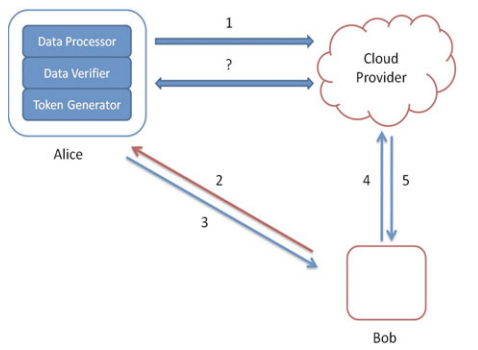
\includegraphics[width=0.6\textwidth]{figures/Customer_Architecture.png}
        \caption[Customer Architecture] {Customer Architecture\cite{Kamara2010}}
\end{figure}

The whole process illustrated in this paper is expressed as follows:
\begin{enumerate}
  \item 
  Alice’s data processor prepares the data (encrypted with symmetric searchable encryption) before sending it to the cloud.
  \item 
  Bob asks Alice for permission to search for a keyword.
  \item 
  Alice’s token and credential generators send a token for the keyword and a credential back to Bob.
  \item 
  Bob sends the token to the cloud.
  \item 
  The cloud uses the token to find the appropriate encrypted documents and returns them to Bob.
  \item 
  At any point in time, Alice’s data verifier can verify the integrity of the data.
\end{enumerate}

\section{FileMap}

“FileMap is a file-based map-reduce system for data-parallel computation”\cite{Mfisk2013}. It is designed and implemented around several application scenarios like file-based and data replication. Its idea of data replication mechanism which is similar to RAID4 or RAID5 means the file is split in the physical separated media and stored. Files could be split into segments and stored in different entities which are both logically or physically separated, or a combination of them. For example, to perform secure cloud storage in logical separated entities, certain file could be fragmented into n segments and stored in one provider’s cloud storage service with n identities (i.e., n segments stored in n accounts of Dropbox respectively). While storing files in physical separated entities, as same as the first scenario, files also have to be divided into n segments but the difference is storing them via different cloud storage providers’ services (i.e., n segments stored in Google Drive, Dropbox and SkyDrive separately). Given the fact that some providers providing encrypted storage service like Dropbox, a pseudo searchable encrypted cloud storage prototype with could be made by:
\begin{enumerate}
  \item 
  Regenerate the file and adding indexes information in the metadata and fragment it into index and content segments.
  \item 
  Store the index segments in plain text stored cloud storage service but with better access control mechanism deployed like Google Drive.
  \item
  Store the rest n content segments in n accounts of encrypted cloud storage service like Dropbox.
\end{enumerate}
                                
  %\chapter{Design}

Current storage systems secure data either via encrypting data on the wire, or through data encryption on the physical disk\cite{ErikRiedelMaheshKallahalla2002}. Cryptographic protection of single file instances could prevent data modification or leakage during storage\cite{Vaquero2010}. Secure Dropbox is designed as a client end encryption tool over the Dropbox service. The main idea is providing a file encryption service with symmetric cryptography where key is not known to Dropbox and, in the meantime, the file encryption key is well protected with asymmetric cryptography for secure file sharing. It is proposed to strengthen the way in which the Dropbox protects users’ file content security from attacks especially those from internal Dropbox. Internal attack is theoretically easy to be performed as Dropbox encrypts those files with keys known to them. Also the security against external attack has been fortified since files will be encrypted twice, Dropbox and Secure Dropbox respectively. Secure Dropbox is proposed to be a C/S architecture system. The server end will work as a key management service (KMS) which mainly processes key management requests and storage request while the client end running on a user's host computer will perform cryptographic computations which are resource consuming. Secure Dropbox performs file operations like uploading, downloading and sharing via Dropbox API or the Dropbox official client which is essentially built with Dropbox API as well. The user interface of Secure Dropbox will be designed as a file system operation interface. Encryption within this service will be transparent to the users. The very security of Secure Dropbox service is based on user’s proper usage of Secure Dropbox account information. Two application modes will be provided: using regular mode when there is Internet access while in local mode when there is no Internet access. The different operation permission schema is granted to users.

\begin{figure}[h]
        \centering
        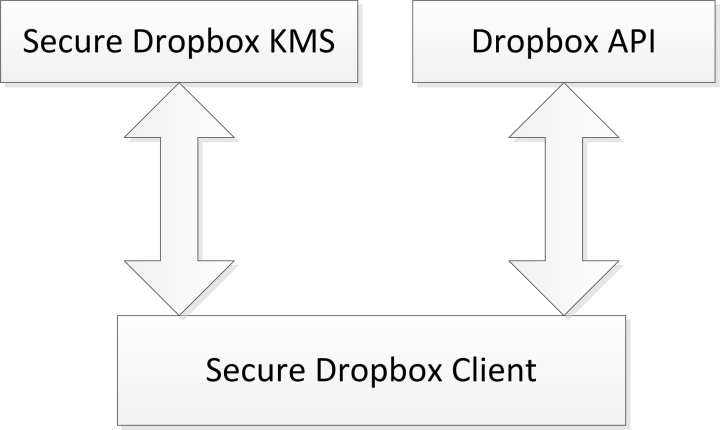
\includegraphics[width=0.6\textwidth]{figures/Secure_Dropbox_Architecture.png}
        \caption[Secure Dropbox Architecture] {Secure Dropbox Architecture}
\end{figure}

This chapter will discuss some major design decisions and implementation challenges during the Secure Dropbox project. Firstly, the overall design of Secure Dropbox will be proposed. Secondly, the cryptography application mechanism to guarantee the security of Secure Dropbox will be explained and justified. Furthermore, the reason for making choices about ways of performing file operations, systematic integration with Dropbox and a platform on which to construct the application will be discussed in regard to building a platform independent application. Moreover, the decisions made in terms of building a C/S architecture application but not in B/S architecture will be explained. Some other design features are more intuitively understandable by explaining from the implementation aspect so more detail of those parts will be proposed in the next chapter or just briefly mentioned in this chapter. Lastly, the design decisions and other principles proposed to implement Secure Dropbox are not Dropbox oriented specifically but could be adopted when designing any application that protect users file in the cloud and provide a reliable file sharing in the cloud storage system.

\section{Application of Cryptography}

Dropbox claim that they are using Secure Socket Layer (SSL) on data transmission and performing AES 256-bit encryption with users’ data. It seems sufficient against external attack but only on condition that the attacking does not come to key management service (KMS). However, these mechanisms make no sense of protecting users’ data from internal attack, which is performed by employees of Dropbox who have access permission to KMS. The behavior, or say the ability, of accessing to users’ data has been admitted in their terms of service\cite{Dropbox2012} that Dropbox will remove the encryption from file data and deliver them to law enforcement on government’s requirement. Nevertheless, because of internal attacker’s proficient understanding of Dropbox system and some inappropriate access permission configurations, internal attacks could even be done unconsciously. These security concerns have been certified that several internal attack events are reported. Client end encryption is one of those alternatives recommended by Dropbox if users are more willing to conceal their data and care less about losing some Dropbox features like version control or data recovering\cite{Dropbox2012}. More importantly, when protecting user’s data from internal Dropbox attack with client end encryption, it actually disables the file sharing infrastructure provided by Dropbox totally.

Anyway, cryptography is still going to be the very insurance for the security of Secure Dropbox. Generally, Secure Dropbox is designed to make Dropbox internal attack impossible and also to provide a cipher file sharing service. To achieve this goal, Secure Dropbox will apply a combination of symmetric cryptography and asymmetric cryptography. The symmetric cryptology like AES or DES will be used for file content encryption given the fact that they are much faster than asymmetric cryptography and sufficient security offered. The asymmetric cryptology is used for protecting the symmetric encryption key and providing a secure key transmission service. In the following example, the procedure of secure storage is going to be illustrated with AES and RSA as instance of symmetric and asymmetric cryptography respectively:

\begin{figure}[h]
        \centering
        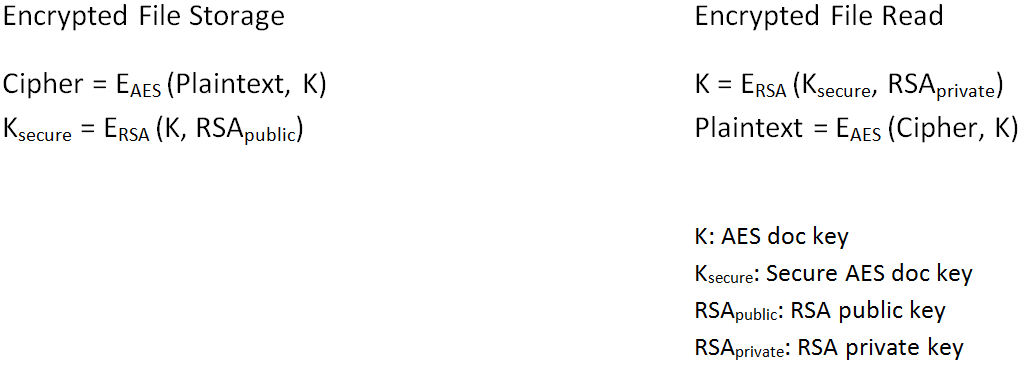
\includegraphics[width=1.0\textwidth]{figures/Encrypted_File_Storage_&_Reading.png}
        \caption[Encrypted File Storage and Reading] {Encrypted File Storage and Reading}
\end{figure}

In the file encrypted storage procedure, plain text is ciphered in AES with a random generated AES file encryption key. The doc key is later ciphered in RSA as well with file owner’s RSA public key.
In encrypted file read procedure, firstly the ciphered doc key $K_{secure}$ should be deciphered in RSA with file owner’s RSA private key. Having retrieved the raw doc key K, the cipher could be decrypted in AES with K.
The procedures of sharing from Secure Dropbox users is mainly about ciphering the doc key K and transferring it to the sharing recipient. K should be ciphered by file owner but could only to be deciphered by sharing recipient, which is a typical scenario for asymmetric cryptography application. In the following example, Alice wants to share a file with Bob:

\begin{figure}[h]
        \centering
        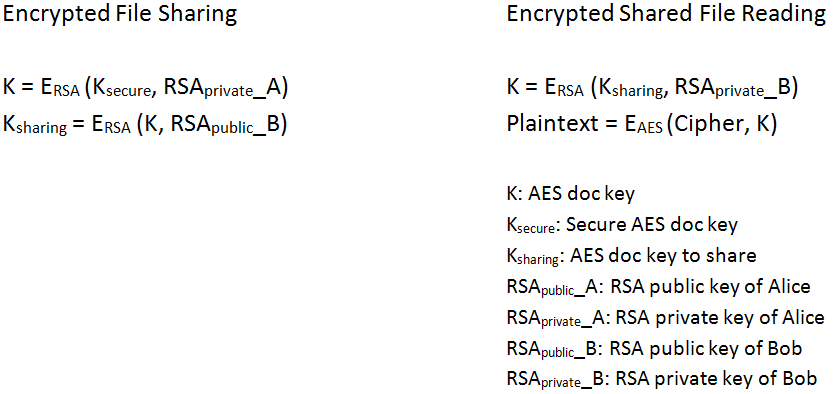
\includegraphics[width=1.0\textwidth]{figures/Encrypted_File_Sharing.png}
        \caption[Encrypted File Sharing] {Encrypted File Sharing}
\end{figure}

Sharing procedure as shown above actually does not perform any operation on the file instance but only cipher the key for sharing purpose. The doc key is stored in a secure way at the very beginning. To get the raw doc key, Alice has to decipher $K_{secure}$ in RSA with her own RSA private key. In order to enable Bob deciphering the key ciphered by Alice, she should encrypt the raw doc key K in RSA with Bob’s RSA public key, which is open to all the users in the Secure Dropbox system. $K_{sharing}$ is generated in this way and then transmitted to Bob via secure tunnels. After receiving the $K_{sharing}$, Bob will decrypt it in RSA with his own RSA private key and then get the raw doc key. Now the plain text of the shared encrypted file could be retrieved by decrypting in AES with the raw doc key.

Respecting managing the RSA key pair of Secure Dropbox user and doc key of each file, a detailed design description will be given in the coming section.


\section{Key Management Service}

In the Secure Dropbox application scenario, there should be an infrastructure posting all Secure Dropbox users’ RSA public key for sharing sponsor to achieve during the encrypted file sharing procedure. In addition, given the essence of Secure Dropbox (a client end file encryption tool) and Dropbox’s cloud storage nature, the requirement of everywhere use should be met. It means as long as users could get access to Dropbox, they are allowed to use the Secure Dropbox service like downloading the desired doc key chain and RSA key pairs. To achieve the goal, besides generating a local copy of essential data like Secure Dropbox users’ authentication information, RSA key pairs, doc keys and file sharing information, these records should also be stored on a server which is able to be accessed anytime anywhere.

Dropbox stores file encryption key in its own database makes it not an accredited storage service to users. However, in order to avoid same security concerns towards Dropbox about its encryption mechanism, some improvements should be made. To make Secure Dropbox reliable, the authority of decrypting file should be only granted to owner but no one else even the KMS administrator. A possible alternative is storing all sensitive data (e.g. RSA private key and doc key) on the server confidentially so that the everywhere usage could be realized safely. Therefore, the only entry (assume it could be something like an access token or password) of decrypting all these sensitive data should never be stored on the server but only held by users themselves.

\begin{figure}[h]
        \centering
        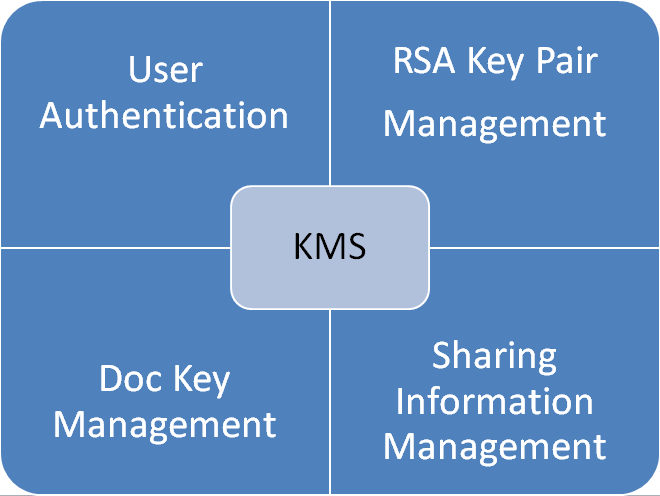
\includegraphics[width=0.6\textwidth]{figures/KMS_Architecture.png}
        \caption[KMS Architecture] {KMS Architecture}
\end{figure}

\subsection{KMS User Authentication}

User authentication information is a basic component in any web application instance as long as access control is required. The classic way applied in web application saves user’s authentication could be adopted: for the minimum usage, a plain text username and a hashed password should be saved. The authentication procedure will match the username and password hash value. The hashed password is generated in the client and only the hash value with algorithm indicator prefixes will be uploaded to KMS and stored. To avoid performing any suspicious behavior, plain text password should be hashed in client once it is received in the terminal and uploaded for authentication. There is no plain text password involves in the KMS server end. The hash value matching could be done at client as well but it requires a corresponding KMS interface for users to fetch hash algorithm’s salt, iteration times and hash value.

\subsection{KMS RSA Key Pair Management}

The RSA key pair could be generated either on KMS or client although it would potentially bring about better user confidence when everything is generated in the client and uploaded after encryption. In KMS, RSA public key is stored in plain text so that it could be reached by any user who wants to process the doc key before sharing the file. An RSA private key should be stored in cipher. It is encrypted in symmetric cryptography with user’s own password or token as encryption key and uploaded once generated in client end. Any request about fetching Secure Dropbox users’ RSA public key should be allowed.

\subsection{KMS Doc Key Management}

For each file encrypted by Secure Dropbox, a unique file encryption key will be generated. Before uploading to KMS, it is a necessity to encrypt the doc key in RSA with file owner’s RSA public key. The document’s name will be stored in plain text for easy indexing purpose. In this way, any operation on this encrypted file, no matter reading or sharing, could only be initiated by the file owner. It is because both procedures require file encryption key that is only known to file owner. The RSA private key is involved in decryption in corresponding to the encryption with RSA public key that from the same key pair.

\subsection{KMS Sharing Information Management}

The key component of sharing data is still the processed doc key. The processing procedure should be performed on the client. The sharing recipient will be able to get the processed key and decrypt it with own RSA private key. Besides it should include sharing metadata generated by Dropbox sharing API: a URL indicates the entry of the file content and a sharing expiration timestamp indicates when the URL will be closed for access.

\subsection{Local KMS}

There are two modes for Secure Dropbox: regular mode when Internet access is available and a local mode when Internet access is not available. A local copy of KMS information related to the Secure Dropbox user is generated for local usage like providing user authentication information, RSA key pair information and file encryption keychain. Since there is no Internet access, User can neither share a file with other Secure Dropbox users nor read shared files from other Secure Dropbox user. User’s own files stored in the local file system are still accessible given the design decision made about using the Dropbox official application as file container. The local RSA key pair and doc keychain make it possible to decrypt any encrypted files. Apparently this local copy should be protected and encrypted as well.

\section{Right Cryptography Algorithm}

\subsection{Symmetric Cryptography}

In the symmetric (private-key) cryptography procedure, encryption and decryption are performed with same key\cite{Bellare1997}. Accordingly, encryption key sharing becomes the precondition of the sharing the symmetrically encrypted information. Theoretically, as it is significantly faster in comparison with asymmetric algorithm with the same security level, symmetric encryption algorithm is usually used for big data protection.

Advanced Encryption Standard (AES) is a specification for the encryption of electronic data established by the U.S. National Institute of Standards and Technology (NIST) in 2001\cite{Information2001}. NIST claimed that AES with 128-bit keys provides adequate protection for classified information up to the SECRET level definition. Increasing AES applications have changed to the AES-256 in which more rounds hash and longer key are applied and fulfill a TOP SECRET level by definition (Both definitions of SECRET and TOP SECRET are advised by CNSSP-15\cite{National2003}). Numerously there are 3.4 $\times$ $10^{38}$ combinations to guess for AES-128 while this number is squared and comes to an incredible 1.1 $\times$ $10^{77}$ for AES-256.

As Dropbox is using AES-256 for encryption in transit and encryption in rest, seemingly it would be ideal to deploy an AES-256 encryption in Secure Dropbox for file encryption as well. As claimed by NIST\cite{Publication2007}, the encryption strength of AES-256, which has an equivalent security level as RSA-15360, will be sufficient until 2030. In Secure Dropbox, AES-256 will be the most direct protection of all data include encrypted file storage, encrypted local storage of user’s file encryption key chains and other confidential data in server end as long as content concealing is required.

However, since the guaranteed security totally depends on a proper key usage and storage, it is highly risky to transmit the unprotected file encryption key via unreliable media like the Internet. So, despite of those application layer protocols for secure data transmission like SSL, hybrid encryption which combines the symmetric encryption and asymmetric encryption would be a better way to directly protect the symmetric encryption key against risks during key exchange.

\subsection{Asymmetric Cryptography}

Practically, the security of cryptography nowadays is no longer guaranteed by concealing the cryptography algorithm itself but lies on the encryption key strength and mechanism of key protection. While sharing the symmetrically encrypted data will inevitably involve key exchange on unreliable public tunnels where interception and distortion are happening, the asymmetric cryptography turns out to be a better option.

In asymmetric cryptography, the encryption and decryption are performed with mathematically linked public key and private key respectively. Generally speaking, the public key is for encrypting the plain text while the private key is used for decryption purpose. The key pair is generated by a trusted PKI. The key pair, especially the private key, is distributed far less often than symmetric encryption application scenario. It essentially reduces the security threats brought by frequent key exchange. As a prerequisite of encrypted information sharing, the public encryption key is widely distributed and accessible by anyone who wants to activate information sharing. However, the private key will be only known to the encrypted information recipient. As a result, there is only transmission of encrypted data which could be considered as secure rely on the strength of asymmetric cryptography algorithm and its key length.

Nevertheless, due to the different mathematical natures in comparison with symmetric cryptography, asymmetric algorithm is remarkably less efficient. Most applications of asymmetric cryptography are limited to small data encryption or as a component in hybrid encryption. For example, to share a large encrypted data, the data content is encrypted in the faster symmetric cryptography such as AES while the relatively short AES key is protected with asymmetric cryptography before transmission.

RSA is an algorithm for asymmetric cryptography based on the presumed difficulty of factoring large integers. As claimed by RSA Security, there is a mapping relationship of security strength between RSA and AES in terms of the encryption key length. The correspondence is listed as follows:

\begin{figure}[h]
        \centering
        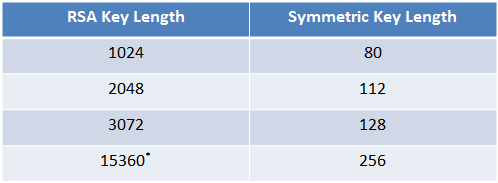
\includegraphics[width=0.7\textwidth]{figures/Strength_Equivalence.png}
        \caption[Strength Equivalence] {Strength Equivalence\cite{Kaliski2009}\cite{Publication2007}}
\end{figure}

RSA Security also claimed that 1024-bit keys are likely to become unsafe sometime between 2006 and 2010 while the 2048-bit keys are sufficient until 2030. Thus the RSA key length of 3072 bits will be required since 2030\cite{Kaliski2009}. RSA with 2048-bit or longer key should meet the requirement of file encryption key security of Secure Dropbox.

\subsection{Cryptographic Hash Function}

Cryptographic hash functions perform irreversible encryption on an arbitrary length plain text and returns a fixed length cipher. The hash digest is fixed for same input but tremendously changed as long as changes happen to content, no matter how trivial it is\cite{Merkle1990}. These one-way hash functions provide a rapid method for detecting any change made to the content and are also used for generating individual digest of content\cite{Merkle1990}. In web application context, user’s confidential information is usually stored in the form of hash digest in case of being exposed when server is exploited.

Since the hash function by definition has the same output with the same input, hash collision attack is easy to perform. For example: Alice sets her password as ``123456'' while Bob coincidentally sets his password as ``123456'' too. Consequently, same password hash values will be generated and stored. If Alice happens to get the password hash table that stored in the server, she might recognizes that Bob’s password hash value is exactly the same with hers and further realizes that Bob’s plain text password could be the same as Alice’s:

\begin{figure}[h]
        \centering
        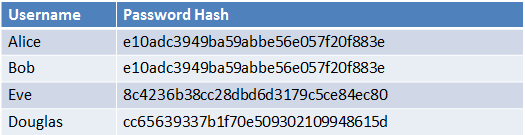
\includegraphics[width=0.8\textwidth]{figures/Hash_Table.png}
        \caption[Hash Table] {Hash Table}
\end{figure}

Also, if Alice has the dictionary of most frequently used password, she could try to hash each password in the collection and match to see if the same hash value exists. Accidentally she might find that Eve’s hashed password could be achieved by hashing ``654321'' with certain algorithm.

To protect the password hash value against hash collision attack, a random generated salt and configurable hash function iteration time could be applied when performing the content hashing. Randomly generated salt acts as a part of content to make same content distinct. The stored hash value is the result of hashing the combination of primary content and salt. Also the adoption of different iteration with different round times leads to a more sophisticated mapping relationship between plain text and hash value. The following example illustrates how a hash table with salt and iteration information stored in the server:

\begin{figure}[h]
        \centering
        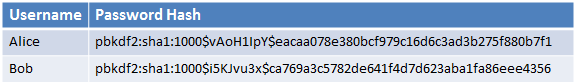
\includegraphics[width=0.9\textwidth]{figures/Hash_Table_with_Salt_Iteration_and_Algorithm_Indicated.png}
        \caption[Hash Table with Parameters] {Hash Table with Salt, Iteration and Algorithm Indicator}
\end{figure}

As shown above, there is additional information attached to the hash value. Take first record for example:

\begin{itemize}
  \item
  pdkdf2 indicates the library’s name via which the hash algorithm is used.
  \item
  sha1 indicates the algorithm used to generate the hash value.
  \item
  1000 indicates there are 1000 iterations when performing the password hashing.
  \item
  ``vAoH1lpY'' is the salt added to the plain text password before it is hashed.
\end{itemize}
		
The hash value to be matched should be generated with the above parameters. In this example, the SHA1 generates a 160-bit long digest of the content. It could be considered as a sufficient secure hash function since it is still widely used in mainstream security protocols like TLS and SSL.

\section {Integration with Dropbox}

Dropbox provides several kinds of APIs for Dropbox developers. For example, The Dropbox Core API, which is recommended as an ideal API set by Dropbox for server-based applications with programming interface for file reading and writing provided. It is also claimed as the most direct way to access Dropbox. Furthermore, it includes some advanced functionality interfaces like content search, version control and restoring file service for developers to performing low-level controls. The Dropbox Sync API, which provides file system-similar programming interface, encapsulates functionality implementations like synchronizing and notification of remote changes. It mainly orients to mobile platform programming. With respect to implementing Secure Dropbox, not only file synchronization operation like uploading and downloading, but also some low-level operations like file sharing, sharing URL generation and file metadata checking are required. To use Dropbox Core APIs, an access token obtained during Dropbox OAuth is essential. The access token will allows Secure Dropbox, a third-party application, to use the Dropbox API with granted permission but never get disclosed with any Dropbox user account information. The implementation details about how to perform the indirect authentication will be proposed in the implementation chapter. Some key Dropbox Core APIs are listed as follows:

\begin{figure}[h]
        \centering
        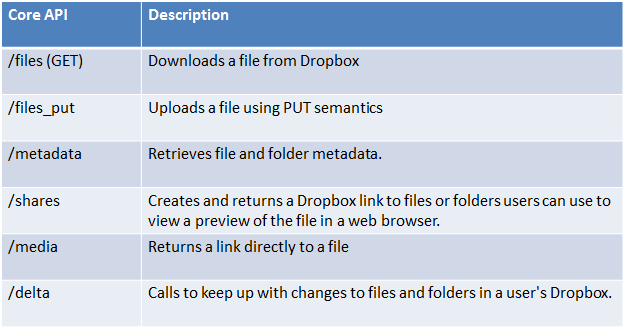
\includegraphics[width=0.9\textwidth]{figures/Key_Dropbox_Core_APIs_Functionality_Description.png}
        \caption[Dropbox Core API] {Key Dropbox Core APIs Functionality Description}
\end{figure}

Except exploiting these Dropbox APIs as advised, there is another way to use Dropbox service – synchronizing files through the Dropbox official application. Using Dropbox on the host computer is just like using any other folder in the file system. However, the files you drag or copy into Dropbox folder will be automatically synchronized and consequently synchronized to other terminals like mobile devices which are linked to Dropbox account. In this way, the Core API is still used but indirectly because the underlying interface for Dropbox official applications is implemented in Core API. The story with regard to file operation could be tremendously simplified if Secure Dropbox use the Dropbox client application as target folder and perform all file operations on it. Correspondingly, every encrypted file written into the Dropbox client folder will be uploaded automatically but without any Dropbox API invoked explicitly. A commercial software product with the same design and implementation relating to the hybrid usage of Dropbox APIs is Boxcryptor\cite{BoxCryptor2013}. Boxcryptor has a driver level encryption which is more efficient than user space encryption. However, the nature of client end encryption disables the sharing service infrastructures provided by Dropbox since file shared that way would be nonsense to human reader since the data is encrypted. Boxcryptor made their own sharing service which partially depends on Dropbox core API service like getting raw content of encrypted file via ``/media'' interface and sharing after decryption.

Although the Dropbox client folder eases the complexity when design the file operation module of Secure Dropbox, the file sharing feature of Dropbox client has been disabled. To analyze from API invoking’s perspective, ``/share'' function of Dropbox core API returns the URL refers to file or folder entity encapsulated with html information so there could be a rendered display of certain entity while the ``/media'' function returns the URL refers to a raw file content text. Apparently, if a file has been encrypted by Secure Dropbox and uploaded to Dropbox, it would be accessible by authenticated user but not meaningful until these encrypted data have been through the decryption service provided by Secure Dropbox. A potential solution to such a problem is a combination usage of Dropbox client and Dropbox API. For instance, the shared information could be accessed by firstly get the encrypted raw data via ``/media'' interface and decrypted in Secure Dropbox while other synchronization operations are still based on the Dropbox application. Another concern derives from the lack of access controls on Dropbox official application. The permission to use Dropbox application is incorrectly granted in the following scenario: Alice logins to Secure Dropbox service with her Secure Dropbox account and performs some file operations at her laptop. Bob comes to Alice and asks for a temporary use. When Bob logins with his Secure Dropbox account and uses Secure Dropbox, the file operations are actually performed on Alice’s Dropbox account. Dropbox does not open API to reset the Dropbox client account information of Dropbox application.

\section{C/S or B/S}

As so long as there is a cryptographic operation happens in the server end, there will be encryption key involved inevitably. It also potentially indicates that the server is allowed to do anything with the encryption key like storing or distributing it. So, to make Secure Dropbox security confident to users, KMS of Secure Dropbox will not be allowed to involve any cryptography procedure. Apparently a B/S architecture, where client is designed to be light while the server is fully responsible for all computations, will not be considered as a reasonable decision. It could be the foremost reason why a C/S designed architecture is more appropriate. However, to reduce the workload of server, in C/S architecture client is assigned with more tasks. Also only the processed data will be submitted to the server. Besides the key involvement issue, in Secure Dropbox the cryptography is the most resource consuming procedure especially when data to be processed is huge. All these tasks done by Secure Dropbox client end could significantly reduce the server’s workload. Based on this design, KMS’s work has been simplified to only process IO requests and perform local storage procedure. Where the encryption potentially involved in Secure Dropbox is illustrated as follows:

\begin{figure}[h]
        \centering
        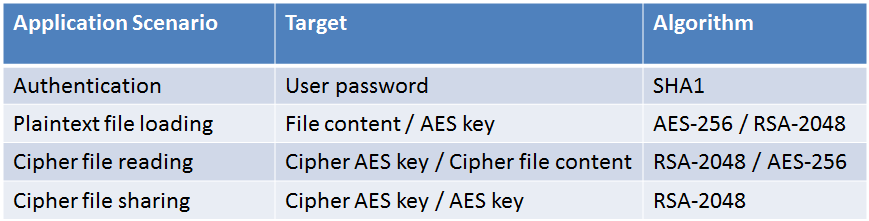
\includegraphics[width=0.9\textwidth]{figures/Cryptography_Application_Scenarios_in_Secure_Dropbox.png}
        \caption[Cryptography Deployment] {Cryptography Application Scenarios in Secure Dropbox}
\end{figure}








  %\chapter{Design}

The design...

  %\chapter{Simulations}

The simulations.

  %\chapter{Conclusion}

This chapter draws some conclusions from evaluation results achieved from user testing session and summarizes some criticisms of the project. The future work planned for the Secure Dropbox is then proposed.

\section{Results}

\subsection{Was An Effective User End Encryption Tool Developed?}

The best approach to appropriately illustrate the idea of user end encryption tools and asymmetric cryptography based secure sharing mechanism is to build a working prototype. Secure Dropbox accomplishes one and the most key ideas in accordance with security have been expressed. Secure Dropbox does not invent anything but applied a cryptography combination in a new application scenario. Its security is based on classic, strict, widely used and universally accepted cryptography algorithm. The design makes it zero-knowledge software: Secure Dropbox never has access to the file or even the encryption keys. Statically stored data that should be kept as secrets are unquestionably stored confidentially. It undeniably gains users’ confidence when using public cloud storage to store their confidential documentations according to the user testing feedbacks. Secure Dropbox users will never work with unencrypted files in their Dropbox which are ready to share with a small conversion upon the encryption key. Secure Dropbox could already be thought as a successful user end encryption tool to some extent.

However, it is still far from being a commercial software product. It provides a higher level of security but at the same time disables some important features of Dropbox. Actually, to most uncommercial users, the stability and fault-tolerance of a cloud storage are often considered as much as security. The trade-off will be absolutely there until these problems have been solved. Now Secure Dropbox is only implemented as prototype.

\section{Criticism}

\subsection{Design Criticism}

Although it explains the main idea of Secure Dropbox, the project is designed only for demonstration purpose. It lacks essential features that could actually make a better idea expression. For example, a logging module is always built in any software. The potential fault-tolerance and error recovering features of Secure Dropbox could have been illustrated by implementing an embedded logging module. It also lacks of consideration about availability such as it was designed to grant user with a minimum file reading permission in Secure Dropbox local mode. Although most timely Dropbox application based synchronization works robustly, no fault recovering or feedback is provided when errors occur. It is because Dropbox application is not designed to be based on by another application so there is no programmable interface provided. Dropbox core API is the only recommended way to implement a third-party application of Dropbox.

\subsection{Implementation Criticism}

The user space cryptography implementation essentially narrows down the supported file types by Secure Dropbox. For this stage only text file is supported and to support a new file type requires considerable efforts. A file system level encryption implementation would solve this problem. Additionally, a more flexible configuration interface should be made like allowing users to configure their own cryptography application schema based on different environment and practical requirements. The user experience should be improved by redesigning the user interface based on some human computer interaction principles and adding practical functionalities. 

\subsection{Testing  Criticism}

Performance testing lacks of comparison with other cryptography algorithms or under different running environment. Consequently these numbers do not speak much about the performance of Secure Dropbox. In addition, the user experience testing lacks of expert participants although some of them have computer science background. Security experts usually have a better understanding in this area and they are able to propose constructive expertise about such a software product.

\section{Future Work}

\subsection{Version Control and File Recovering}

Version control and file recovering service provided by Dropbox is disabled because there is no corresponding file encryption key version control module in Secure Dropbox. A possible design could be padding the file name with a timestamp and using this file name as the key of the version control table. This table records the history of certain file and its corresponding encryption key.

\subsection{User Profile Management}

With reference to user profile management, only the user registration and login have been implemented. The following jobs will be the implementation of a more generic user profile management module with common features like logout, account cancellation and more importantly password modification. The updating mechanism towards the expired RSA key pair which is also a part of user profile will be implemented as well.

\subsection{Improvement of Sharing Mechanism}

The file will keep using the same key until its source text has been modified and reloaded via Secure Dropbox again. For now file sharing does not change the file encryption key because the sharing URL could be cancelled or automatically expires after certain time slot. Also shared files could only be accessed after valid authentication and through Secure Dropbox user interface control. However, a new file sharing mechanism provides one time encryption key which guarantees a better security for the file. The file encryption key has been known to other users will no longer be available after sharing is cancelled.

\subsection{File Sharing Refreshing}

The file sharing URL generated by Dropbox expires in 3 hours. It is consistent with Dropbox OAuth access token because Dropbox does not allow third-party application who holding an expired access token could still access the shared file. To keep the file sharing until further cancellation, the file sharing record in the database should be refreshed periodically to update the previous URL and expiration timestamp. However, calling ``/media'' interface requires a valid token which has to be fetched by playing manual authentication. A proper mechanism of keeping the access token valid will call for more investigations.

\subsection{File System Level Encryption}

Secure Dropbox currently supports operation upon text file only because the implemented user space encryption could play file manipulations conveniently upon text files although it is sufficient as a prototype for demonstration. File system level encryption makes cryptography procedure transparent to user space applications. Dragging files into the specific folder with customized file system level system calls will trigger file encryption automatically and vice versa.

\subsection{Configuration Interface}

Now Secure Dropbox configuration could be carried out by changing parameters in Python source code. While an embedded configuration user interface could limit the options for configuration and execute parameter checking before the new configuration taking effect.

\subsection{Multi-platform Implementation}

There are lots of Dropbox users who want to synchronize their files between different terminals. Since Secure Dropbox is implemented with Python, it would not cost much effort to do the application transplantation between different operating systems. Python is also supported in some portable operating systems like Android and iOS. The difference to be concerned will be mainly about the computation and network capacity which impacts the performance significantly.

\subsection{Better Local KMS Mechanism}

Now Secure Dropbox local mode works based on KMS files stored in local file system which is generated after last login. It provides file encryption keychain and RSA key pair required in order to execute reading operation. Nevertheless, a better designed local KMS mechanism should guarantee Secure Dropbox users the same experience seamlessly as the regular mode does. An optimized local KMS mechanism is designed to perform delay tolerant KMS information updating when Internet access revives. 
  %\chapter{Conclusions}

And a fancy conclusion...



%\addcontentsline {toc}{chapter}{Appendices}       %% Force Appendices to appear in contents
\begin{appendix}
\chapter{Abbreviations}

\begin{tabular}{p{40mm}|p{100mm}}
	\textbf{Short Term}&\textbf{Expanded Term}\\
	\hline
	SaaS&Software as a Service\\
	...&...
\end{tabular}

%\chapter{Task Description}
\begin{enumerate}
  \item
  Please register a Secure Dropbox account with your email address and login with this account.
  \item
  Check the Secure Dropbox folder in Dropbox folder. Open the ini file includes your username with any text editor.
  \item
  Load a text via Secure Dropbox with ``load'' command.
  \item
  Check the Secure Dropbox folder in Dropbox folder again. You will see a file whose file name is made up with the 
  file’s name you just loaded, your account name and end up with suffix enc. Open this file and see if it is encrypted.
  \item
  Use read command in Secure Dropbox to read the file you just loaded.
  \item
  Open another Secure Dropbox client. Register another Secure Dropbox account and login with that account.
  \item
  Back to the first Secure Dropbox client. Use ``share'' command to share the file you just loaded with the new account you just registered.
  \item
  Switch the later opened Secure Dropbox client. Use ``shared'' command to see if there is file shared with you and use ``read shared'' command to read the shared file.
  \item
  Open use. Please do any operation you want with Secure Dropbox. Help information will display by using command ``?''
\end{enumerate}


\end{appendix}


%\addcontentsline {toc}{chapter}{Bibliography}     %% Force Bibliography to appear in contents

%\begin{thebibliography}{ieeetr}                   %% Start your bibliography here; you can
%\bibliography{refs}                               %% also use the \bibliography command
 
%@incollection{kamara2010cryptographic,
  title={Cryptographic cloud storage},
  author={Kamara, Seny and Lauter, Kristin},
  booktitle={Financial Cryptography and Data Security},
  pages={136--149},
  year={2010},
  publisher={Springer}
}



\printbibliography
%\end{thebibliography}                             %% to generate your bibliography.


\end{document}                                    %% END THE DOCUMENT
